\chapter{Johdanto}

Kurssin \emph{Tietorakenteet ja algoritmit} tarkoituksena
on opettaa menetelmiä, joiden avulla voimme ratkaista
\emph{tehokkaasti} laskennallisia ongelmia.
Ohjelmoinnin peruskursseilla olemme keskittyneet
ohjelmointitaidon opetteluun.
Nyt on aika siirtyä askel eteenpäin ja alkaa kiinnittää
huomiota myös siihen, miten nopeasti algoritmit toimivat.

Algoritmien tehokkuudella on suuri merkitys käytännössä.
Esimerkiksi netissä toimiva reittiopas on käyttökelpoinen sen vuoksi,
että se antaa ehdotuksen reitistä heti sen jälkeen, kun olemme
ilmoittaneet, mistä mihin haluamme matkustaa.
Jos reittiehdotusta pitäisi odottaa vaikkapa minuutti tai tunti,
tämä rajoittaisi paljon palvelun käyttöä.

Jotta reittiopas toimisi tehokkaasti, sen taustalla on
hyvin suunniteltu algoritmi.
Tällä kurssilla opimme, kuinka voimme luoda itse vastaavia algoritmeja.
Tutustumme kurssilla sekä algoritmien suunnittelun teoriaan että
käytäntöön -- haluamme ymmärtää syvällisesti, mistä algoritmeissa on kysymys,
mutta myös osata toteuttaa niitä käytännössä.

\section{Mitä algoritmit ovat?}

\index{algoritmi}
\index{syöte}
\index{tuloste}

Algoritmi on toimintaohje, jota seuraamalla voimme ratkaista
jonkin laskennallisen ongelman.
Algoritmille annetaan \emph{syöte} (\emph{input}),
joka kuvaa ratkaistavan ongelman tapauksen,
ja algoritmin tulee tuottaa \emph{tuloste} (\emph{output}),
joka on vastaus sille annettuun syötteeseen.

Tarkastellaan esimerkkinä ongelmaa,
jossa syötteenä on $n$ kokonaislukua sisältävä taulukko ja
tehtävänä on laskea lukujen summa.
Esimerkiksi jos syöte on $[2,4,1,8]$,
haluttu tuloste on 15, koska $2+4+1+8=15$.
Voimme ratkaista tämän ongelman algoritmilla,
joka käy luvut läpi silmukalla ja laskee niiden
summan muuttujaan.

Algoritmin toiminnan esittämiseen on useita mahdollisuuksia.
Yksi tapa on selostaa sanallisesti, kuinka algoritmi toimii,
kuten teimme äsken.
Toinen tapa taas on antaa koodi, joka toteuttaa algoritmin.
Tällöin meidän täytyy valita jokin ohjelmointikieli,
jonka avulla esitämme algoritmin.
Esimerkiksi seuraava Java-koodi kuvaa algoritmin,
joka laskee lukujen summan:

\begin{code}
int summa = 0;
for (int i = 0; i < n; i++) {
    summa += luvut[i];
}
System.out.println(summa);
\end{code}

\index{pseudokoodi}

Voimme myös esittää algoritmin \emph{pseudokoodina}
todellisen ohjelmointikielen sijasta.
Tämä tarkoittaa, että kirjoitamme koodia,
joka on lähellä käytössä olevia ohjelmointikieliä, mutta voimme
päättää koodin tarkan kirjoitusasun itse ja ottaa joitakin vapauksia,
joiden ansiosta voimme kuvata algoritmin mukavammin.
Voisimme esimerkiksi esittää äskeisen algoritmin pseudokoodina seuraavasti:

\begin{code}
summa = 0
for i = 0 to n-1
    summa += luvut[i]
print(summa)
\end{code}

Tässä kirjassa esitämme algoritmeja sekä Java-koodina että pseudokoodina
tilanteesta riippuen.
Käytämme Java-koodia silloin, kun haluamme kiinnittää huomiota siihen,
miten jokin asia toteutetaan tarkalleen Javassa.
Pseudokoodia käytämme taas silloin, kun haluamme kuvata algoritmin yleisen
idean eikä käytetyllä kielellä ole merkitystä.
Taulukko \ref{tab:psekoo} näyttää vertailun kirjan pseudokoodin
ja Java-koodin merkintätavoista.

Tärkeä työkalu algoritmien suunnittelussa on \emph{matematiikka},
jonka avulla voi perustella täsmällisesti,
miksi jokin algoritmi toimii ja käyttää tietyn verran aikaa.
Tutustumme tarvittaviin matematiikan asioihin pikkuhiljaa kirjan aikana.
Kirjan lopussa olevassa liitteessä on lisäksi yhteenveto matematiikan
merkinnöistä ja kaavoista, joita kirjassa käytetään.

\lstnewenvironment{smallcode}[1][]%
{
   \noindent
   \small
   \minipage{0.47\linewidth} 
   \vspace{0.5\baselineskip}
   \lstset{#1,xleftmargin=0pt}}
{\endminipage}

\begin{table}
\center
\begin{tabular}{ll}
pseudokoodi & Java-koodi \\
\hline
\begin{smallcode}[xleftmargin=0pt]
x = 5
t = [1,2,3]
\end{smallcode}
&
\begin{smallcode}
int x = 5;
int[] t = {1,2,3};
\end{smallcode}
\\
\begin{smallcode}[xleftmargin=0pt]
if a == b
    // koodia
\end{smallcode}
&
\begin{smallcode}
if (a == b) {
    // koodia
}
\end{smallcode}
\\
\begin{smallcode}[xleftmargin=0pt]
while a <= b
    // koodia
\end{smallcode}
&
\begin{smallcode}
while (a <= b) {
    // koodia
}
\end{smallcode}
\\
\begin{smallcode}[xleftmargin=0pt]
for i = 1 to n
    // koodia
\end{smallcode}
&
\begin{smallcode}
for (int i = 1; i <= n; i++) {
    // koodia
}
\end{smallcode}
\\
\begin{smallcode}[xleftmargin=0pt]
for i = n to 1
    // koodia
\end{smallcode}
&
\begin{smallcode}
for (int i = n; i >= 1; i--) {
    // koodia
}
\end{smallcode}
\\
\begin{smallcode}[xleftmargin=0pt]
sort(x)
\end{smallcode}
&
\begin{smallcode}
Arrays.sort(x);
\end{smallcode}
\\
\begin{smallcode}[xleftmargin=0pt]
print(x)
\end{smallcode}
&
\begin{smallcode}
System.out.println(x);
\end{smallcode}
\\
\begin{smallcode}[xleftmargin=0pt]
swap(a,b)
\end{smallcode}
&
\begin{smallcode}
t = a; a = b; b = t;
\end{smallcode}
\\
\begin{smallcode}[xleftmargin=0pt]
a = min(x,y)
b = max(x,y)
\end{smallcode}
&
\begin{smallcode}
a = Math.min(x,y);
b = Math.max(x,y);
\end{smallcode}
\\
\begin{smallcode}[xleftmargin=0pt]
procedure toisto(x)
    print(x)
    print(x)
\end{smallcode}
&
\begin{smallcode}
void testi(int x) {
    System.out.println(x);
    System.out.println(x);
}
\end{smallcode}
\\
\begin{smallcode}[xleftmargin=0pt]
function summa(a,b)
    return a+b
\end{smallcode}
&
\begin{smallcode}
int summa(int a, int b) {
    return a+b;
}
\end{smallcode}
\\
\end{tabular}
\caption{Pseudokoodin ja Java-koodin vertailu.}
\label{tab:psekoo}
\end{table}

\section{Ohjelmoinnin peruspalikat}

Kiehtova seikka ohjelmoinnissa on, että monimutkaisetkin algoritmit
syntyvät yksinkertaisista aineksista.
Käymme seuraavaksi läpi ohjelmoinnin peruspalikat,
jotka muodostavat pohjan algoritmien suunnittelulle.

\subsubsection{Muuttuja}

\index{muuttuja}

\emph{Muuttuja} (\emph{variable}) säilyttää algoritmissa tarvittavia tietoja.
Esimerkiksi seuraavassa koodissa on kaksi muuttujaa:

\begin{code}
a = 3
b = 4
print(a+b)
\end{code}

Pseudokoodissa käytäntönä on,
ettei muuttujia tarvitse määritellä vaan
voimme alkaa käyttää niitä suoraan.

\subsubsection{Ehtolause}

\index{ehtolause}

\emph{Ehtolause} (\emph{conditional statement}) saa ohjelman toiminnan
riippumaan muuttujista.
Esimerkiksi seuraava koodi kertoo, onko $x$ parillinen vai pariton:

\begin{code}
if x%2 == 0
    print("parillinen")
else
    print("pariton")
\end{code}

\subsubsection{Silmukka}

\index{silmukka}

\emph{Silmukka} (\emph{loop}) toistaa koodia.
Esimerkiksi seuraava for-silmukka tulostaa luvut $1,2,3,\dots,10$.

\begin{code}
for i = 1 to 10
    print(i)
\end{code}

Seuraava while-silmukka puolestaan puolittaa lukua $x$,
kunnes se on pienempi kuin 1:

\begin{code}
while x >= 1
    print(x)
    x /= 2
\end{code}

\subsubsection{Taulukko}

\index{taulukko}
\index{tietorakenne}

\emph{Taulukko} (\emph{array}) on ohjelmoinnin tavallisin \emph{tietorakenne}
(\emph{data structure})
eli tapa säilyttää kokoelmaa tietoa ohjelmassa.
Taulukossa on $n$ alkiota, joiden kohdat ovat $0,1,\dots,n-1$.

Esimerkiksi seuraava koodi luo taulukon ja käsittelee
sen kohdassa 2 olevaa alkiota:

\begin{code}
x = [4,2,7,5,1]
print(x[2]) // 7
x[2] = 3
print(x[2]) // 3
\end{code}

Seuraava koodi puolestaan tulostaa kaikki
$n$-kokoisen taulukon alkiot:

\begin{code}
for i = 0 to n-1
    print(x[i])
\end{code}

Tutustumme kirjan aikana moniin tietorakenteisiin,
joista on hyötyä algoritmien suunnittelussa.
Pystymme kuitenkin halutessamme toteuttamaan
minkä tahansa tietorakenteen taulukon avulla.
Tämä johtuu siitä, että tietokoneen muisti
on pohjimmiltaan suuri taulukko.

\subsubsection{Aliohjelma}

\index{aliohjelma}
\index{metodi}
\index{proseduuri}
\index{funktio}

\emph{Aliohjelma} (\emph{subprogram}) on ohjelman osa, jota voi kutsua parametreilla.
Javassa aliohjelmasta käytetään nimeä \emph{metodi} (\emph{method}).

Tässä kirjassa käytäntönä on,
että \emph{proseduuri} (\emph{procedure}) on aliohjelma,
joka ei palauta mitään (Javassa \texttt{void}),
ja \emph{funktio} (\emph{function}) on aliohjelma,
jolla on palautusarvo.

Esimerkiksi seuraava proseduuri tulostaa kahdesti parametrinsa:

\begin{code}
procedure toisto(x)
    print(x)
    print(x)
\end{code}

Seuraava funktio puolestaan palauttaa
parametriensa summan:

\begin{code}
function summa(a,b)
    return a+b
\end{code}

\subsubsection{***}

Olemme nyt käyneet läpi ainekset,
joiden avulla voimme toteuttaa \emph{minkä tahansa} algoritmin.
On huojentava tieto, että näinkin pieni määrä tekniikoita
riittää algoritmien suunnittelussa.
Nyt kaikki on vain kiinni siitä, miten osaamme \emph{soveltaa}
näitä tekniikoita eri tilanteissa.

\section{Rekursio}

\index{rekursio}

\emph{Rekursio} (\emph{recursion}) on hyödyllinen ohjelmointitekniikka,
joka jää kuitenkin usein sivurooliin ohjelmoinnin peruskursseilla.
Nyt on aika perehtyä kunnolla siihen,
mitä hyötyä rekursiosta on.
Osoittautuu, että voimme toteuttaa monia algoritmeja
kätevästi rekursion avulla.

Rekursiossa on ideana tehdä aliohjelma, joka kutsuu itseään.
Yksi tapa ajatella rekursiota on, että voimme muuttaa sen avulla
silmukan sarjaksi aliohjelman kutsuja.
Tarkastellaan esimerkkinä seuraavaa silmukkaa:

\begin{code}
for i = 1 to 10
    print(i)
\end{code}

Tämä silmukka tulostaa luvut $1,2,3,\dots,10$.
Voimme toteuttaa samalla tavalla toimivan ohjelman
seuraavasti rekursion avulla:

\begin{code}
procedure testi(x)
    if x > 10
        return
    print(x)
    testi(x+1)
    
testi(1)
\end{code}

Tässä \texttt{testi} on rekursiivinen proseduuri,
jolle annetaan parametrina luku $x$.
Jos $x$ on yli 10, proseduuri ei tee mitään (rekursion loppuehto).
Muuten proseduuri tulostaa luvun $x$ ja kutsuu sitten
itseään parametrilla $x+1$ (rekursiivinen kutsu).
Kun proseduuria kutsutaan parametrilla 1,
se tulostaa luvut $1,2,3,\dots,10$ samalla tavalla kuin aiempi silmukka.

Mutta mitä hyötyä rekursiosta on?
Se selviää seuraavista esimerkeistä,
joissa käytämme rekursiota aidoissa ongelmissa.

\subsection{Osajoukkojen läpikäynti}

\index{osajoukko}

Aloitamme ongelmasta, jossa haluamme käydä läpi
kaikki lukujen $1,2,\dots,n$ \emph{osajoukot}.
Esimerkiksi kun $n=3$, osajoukot ovat
$\emptyset$ (tyhjä joukko), $\{1\}$, $\{2\}$, $\{3\}$,
$\{1,2\}$, $\{1,3\}$, $\{2,3\}$ ja $\{1,2,3\}$.
Osajoukkoja on yhteensä $2^n$,
koska jokaisen luvun kohdalla on kaksi vaihtoehtoa:
se tulee tai ei tule mukaan osajoukkoon.
Esimerkiksi kun $n=3$, osajoukkoja on $2^3=8$.

Seuraava rekursiivinen proseduuri muodostaa lukujen
$1,2,\dots,n$ osajoukot.
Ideana on, että teemme kunkin luvun
kohdalla \emph{päätöksen}, tuleeko se mukaan osajoukkoon vai ei.
Toteutamme tämän niin,
että proseduuri kutsuu itseään molemmissa tapauksissa rekursiivisesti.

\begin{code}
procedure haku(k)
    if k == n+1
        // käsittele osajoukko
    else
        mukana[k] = true
        haku(k+1)
        mukana[k] = false
        haku(k+1)
\end{code}

Proseduurin \texttt{haku} parametri $k$ ilmaisee,
minkä luvun kohtalon päätämme seuraavaksi.
Kutsumme aluksi proseduuria parametrilla $k=1$.
Jos $k=n+1$, olemme saaneet osajoukon valmiiksi
ja voimme käsitellä sen haluamallamme tavalla.
Muuten haaraudumme kahteen osaan sen mukaan,
tuleeko luku $k$ mukaan osajoukkoon vai ei.
Molemmissa tapauksissa kutsumme proseduuria parametrilla $k+1$,
jolloin siirrymme käsittelemään seuraavan luvun.

\begin{figure}
\center
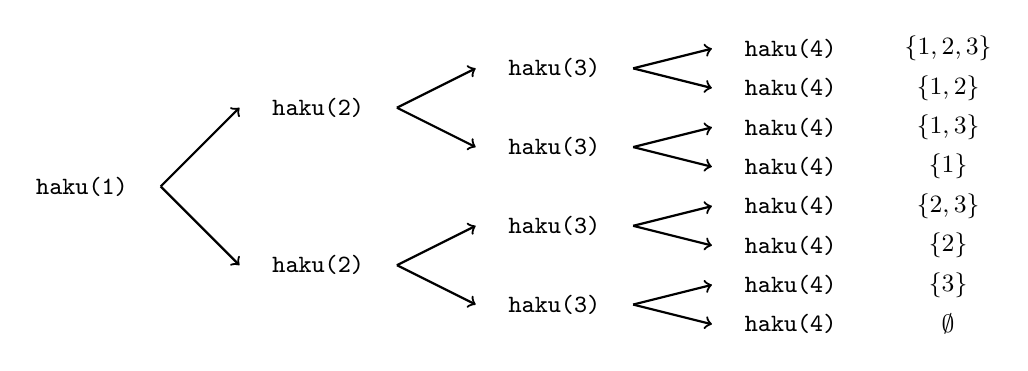
\begin{tikzpicture}[scale=0.5]
\small
\node at (0,0) {\texttt{haku(1)}};
\draw[thick,->] (2,0) -- (4,2);
\draw[thick,->] (2,0) -- (4,-2);
\node at (6.0,2) {\texttt{haku(2)}};
\node at (6.0,-2) {\texttt{haku(2)}};
\draw[thick,->] (8,2) -- (10,3);
\draw[thick,->] (8,2) -- (10,1);
\draw[thick,->] (8,-2) -- (10,-1);
\draw[thick,->] (8,-2) -- (10,-3);
\node at (12.0,3) {\texttt{haku(3)}};
\node at (12.0,1) {\texttt{haku(3)}};
\node at (12.0,-1) {\texttt{haku(3)}};
\node at (12.0,-3) {\texttt{haku(3)}};
\draw[thick,->] (14,3) -- (16,3.5);
\draw[thick,->] (14,3) -- (16,2.5);
\draw[thick,->] (14,1) -- (16,1.5);
\draw[thick,->] (14,1) -- (16,0.5);
\draw[thick,->] (14,-1) -- (16,-0.5);
\draw[thick,->] (14,-1) -- (16,-1.5);
\draw[thick,->] (14,-3) -- (16,-2.5);
\draw[thick,->] (14,-3) -- (16,-3.5);
\node at (18.0,3.5) {\texttt{haku(4)}};
\node at (18.0,2.5) {\texttt{haku(4)}};
\node at (18.0,1.5) {\texttt{haku(4)}};
\node at (18.0,0.5) {\texttt{haku(4)}};
\node at (18.0,-0.5) {\texttt{haku(4)}};
\node at (18.0,-1.5) {\texttt{haku(4)}};
\node at (18.0,-2.5) {\texttt{haku(4)}};
\node at (18.0,-3.5) {\texttt{haku(4)}};
\node at (22.0,3.5) {$\{1,2,3\}$};
\node at (22.0,2.5) {$\{1,2\}$};
\node at (22.0,1.5) {$\{1,3\}$};
\node at (22.0,0.5) {$\{1\}$};
\node at (22.0,-0.5) {$\{2,3\}$};
\node at (22.0,-1.5) {$\{2\}$};
\node at (22.0,-2.5) {$\{3\}$};
\node at (22.0,-3.5) {$\emptyset$};
\end{tikzpicture}
\caption{Osajoukkojen muodostaminen rekursiivisesti ($n=3$).}
\label{fig:osajou}
\end{figure}

Proseduuri merkitsee globaaliin taulukkoon \texttt{mukana},
mitkä luvut ovat mukana osajoukossa.
Voimme hyödyntää tämän taulukon sisältöä,
kun käsitte\-lemme osa\-joukon tapauksessa $k=n+1$.
Esimerkiksi voimme tulostaa osajoukossa olevat luvut seuraavasti:

\begin{code}
for i = 1 to n
    if mukana[i]
        print(i)
\end{code}

Kuva \ref{fig:osajou} näyttää,
miten osajoukot muodostuvat tapauksessa $n=3$.
Jokaisessa proseduurin kutsussa ylempi haara ottaa luvun mukaan osajoukkoon
ja alempi haara ei ota lukua mukaan osajoukkoon.
Kuvan oikeassa reunassa näkyy kussakin tapauksessa muodostettu osajoukko.

\subsection{Permutaatioiden läpikäynti}

\index{permutaatio}

Tarkastellaan sitten toista ongelmaa, jossa haluammekin
käydä läpi lukujen $1,2,\dots,n$ \emph{permutaatiot}
eli kaikki mahdolliset tavat asettaa luvut johonkin järjestykseen.
Esimerkiksi tapauksessa $n=3$ permutaatiot ovat
$(1,2,3)$, $(1,3,2)$, $(2,1,3)$, $(2,3,1)$, $(3,1,2)$ ja $(3,2,1)$.
Luvuista $1,2,\dots,n$ voi muodostaa kaikkiaan $n!$ permutaatiota.
Esimerkiksi tapauksessa $n=3$ permutaatioiden määrä on
$3!=6$.

Myös permutaatioiden läpikäynti onnistuu kätevästi rekursiolla.
Ideana on valita joka askeleella permutaation loppuun
jokin luku, joka ei vielä kuulu siihen.
Voimme toteuttaa haun näin:

\begin{code}
procedure haku(k)
    if k == n+1
        // käsittele permutaatio
    else
        for i = 1 to n
            if not mukana[i]
                mukana[i] = true
                permutaatio[k] = i
                haku(k+1)
                mukana[i] = false
\end{code}

Parametri $k$ tarkoittaa, mihin permutaation kohtaan
valitsemme seuraavaksi luvun.
Haku alkaa, kun kutsumme proseduuria parametrilla $k=1$.
Jos $k=n+1$, olemme saaneet permutaation valmiiksi
ja voimme käsitellä sen.
Muuten valitsemme permutaation kohtaan $k$ tulevan luvun
käymällä läpi silmukalla luvut $1 \dots n$.
Taulukko \texttt{mukana} kertoo, mitkä luvut
ovat jo mukana permutaatiossa
Jos luku $i$ ei ole vielä mukana, haaraudumme tapaukseen,
jossa valitsemme sen kohtaan $k$, ja jatkamme hakua kohtaan $k+1$.

Kun olemme saaneet permutaation valmiiksi,
voimme käsitellä sen esimerkiksi tulostamalla lukujen
järjestyksen näin:

\begin{code}
for i = 1 to n
    print(permutaatio[i])
\end{code}

\subsection{Peruuttava haku}

\index{peruuttava haku}

\emph{Peruuttava haku} (\emph{backtracking}) on yleinen rekursiivinen menetelmä,
jota käyttäen voimme muodostaa kaikki ratkaisut
annettuun ongelmaan.
Ideana on aloittaa tyhjästä ratkaisusta ja käydä
joka askeleella läpi rekursiivisesti kaikki mahdolliset tavat,
kuinka ratkaisua voi laajentaa.

Peruuttava haku on raa'an voiman algoritmi,
ja voimme käyttää sitä vain silloin,
kun ratkaisujen määrä on niin pieni,
että ehdimme käydä läpi kaikki ratkaisut.
Kuitenkin jos voimme käyttää peruuttavaa hakua,
se on mainio tekniikka,
koska voimme olla varmoja, että oikein toteutettu
peruuttava haku löytää kaikki ratkaisut.

\index{latinalainen neliö}

Tarkastellaan esimerkkinä tehtävää, jossa haluamme käydä läpi
kaikki kokoa $n \times n$ olevat \emph{latinalaiset neliöt}
eli ruudukot, joissa kullakin vaaka- ja pystyrivillä
esiintyy tarkalleen kerran jokainen luku $1,2,\dots,n$.
Kyseessä on siis yksinkertaistus tutusta sudoku-tehtävästä.
Esimerkiksi kuva \ref{fig:latnel} näyttää kaikki 12 latinalaista neliötä kokoa $3 \times 3$.

Toteutamme peruuttavan haun niin, että valitsemme joka askeleella
ruudukon kohtaan $(y,x)$ tulevan luvun.
Numeroimme ruudukon vaaka- ja pystyrivit kokonaisluvuin $1,2,\dots,n$.
Aloitamme haun ruudukon vasemmasta yläkul\-masta ja etenemme
rivi kerrallaan alaspäin.
Seuraava rekursiivinen algoritmi toteuttaa haun,
kun sitä kutsutaan parametreilla $(1,1)$:

\begin{code}
procedure haku(y,x)
    if y == n+1
        // käsittele ratkaisu
    else if x == n+1
        haku(y+1,1)
    else
        for i = 1 to n
            if not vaaka[y][i] and not pysty[x][i]
                vaaka[y][i] = pysty[x][i] = true
                nelio[y][x] = i
                haku(y,x+1)
                vaaka[y][i] = pysty[x][i] = false
\end{code}

Algoritmin alussa on kaksi erikoistapausta:
jos $y=n+1$, olemme saaneet muodostettua
yhden latinalaisen neliön.
Jos taas $x=n+1$, olemme saaneet jonkin vaakarivin
valmiiksi ja alamme muodostaa seuraavaa vaakariviä.
Muuten kyseessä on perustapaus, jossa haluamme
valita kohtaan $(y,x)$ tulevan luvun.
Käymme läpi kaikki mahdolliset tavat for-silmukalla,
jossa $i$ on valittava luku.
Koska jokainen luku saa esiintyä vain kerran kullakin
vaaka- ja pystyrivillä, käytämme kahta aputaulukkoa:
$\texttt{vaaka}[y][i]$ kertoo, onko vaakarivillä $y$
jo lukua $i$, ja vastaavasti $\texttt{pysty}[x][i]$ kertoo,
onko pystyrivillä $x$ jo lukua $i$.
Jos voimme sijoittaa luvun $i$ kohtaan $(y,x)$,
merkitsemme tämän taulukkoon $\texttt{nelio}[y][x]$
ja lisäksi päivitämme taulukoita $\texttt{vaaka}$ ja $\texttt{pysty}$.
Sitten jatkamme hakua rekursiivisesti seuraavaan
oikealla olevaan ruutuun.

\begin{figure}
\center
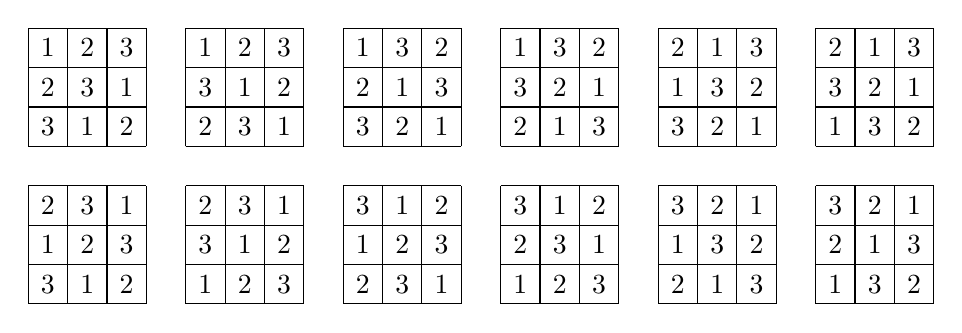
\begin{tikzpicture}[scale=0.5]
\newcommand\nelio[9]{
\draw (0,0) grid (3,3);
\foreach \x/\y/\v in {0/0/#1,1/0/#2,2/0/#3,0/1/#4,1/1/#5,2/1/#6,0/2/#7,1/2/#8,2/2/#9} \node at (0.5+\x,2.5-\y) {\v};
}
\begin{scope}
\nelio{1}{2}{3}{2}{3}{1}{3}{1}{2}
\end{scope}
\begin{scope}[xshift=4cm]
\nelio{1}{2}{3}{3}{1}{2}{2}{3}{1}
\end{scope}
\begin{scope}[xshift=8cm]
\nelio{1}{3}{2}{2}{1}{3}{3}{2}{1}
\end{scope}
\begin{scope}[xshift=12cm]
\nelio{1}{3}{2}{3}{2}{1}{2}{1}{3}
\end{scope}
\begin{scope}[xshift=16cm]
\nelio{2}{1}{3}{1}{3}{2}{3}{2}{1}
\end{scope}
\begin{scope}[xshift=20cm]
\nelio{2}{1}{3}{3}{2}{1}{1}{3}{2}
\end{scope}
\begin{scope}[yshift=-4cm]
\nelio{2}{3}{1}{1}{2}{3}{3}{1}{2}
\end{scope}
\begin{scope}[yshift=-4cm,xshift=4cm]
\nelio{2}{3}{1}{3}{1}{2}{1}{2}{3}
\end{scope}
\begin{scope}[yshift=-4cm,xshift=8cm]
\nelio{3}{1}{2}{1}{2}{3}{2}{3}{1}
\end{scope}
\begin{scope}[yshift=-4cm,xshift=12cm]
\nelio{3}{1}{2}{2}{3}{1}{1}{2}{3}
\end{scope}
\begin{scope}[yshift=-4cm,xshift=16cm]
\nelio{3}{2}{1}{1}{3}{2}{2}{1}{3}
\end{scope}
\begin{scope}[yshift=-4cm,xshift=20cm]
\nelio{3}{2}{1}{2}{1}{3}{1}{3}{2}
\end{scope}
\end{tikzpicture}
\caption{Kaikki 12 latinalaista neliötä kokoa $3 \times 3$.}
\label{fig:latnel}
\end{figure}

\begin{table}
\center
\begin{tabular}{rr}
ruudukon koko $n$ & neliöiden määrä \\
\hline
1 & 1 \\
2 & 2 \\
3 & 12 \\
4 & 576 \\
5 & 161280 \\
6 & 812851200 \\
\end{tabular}
\caption{Latinalaisten neliöiden määrät, kun $n=1,2,\dots,6$.}
\label{tab:latnel}
\end{table}

Kun olemme saaneet muodostettua latinalaisen neliön, voimme
tulostaa sen sisällön taulukon \texttt{nelio} perusteella
tai vain kasvattaa laskurin arvoa,
jolloin saamme lasketuksi, montako neliötä on olemassa kaikkiaan.
Taulukko \ref{tab:latnel} sisältää latinalaisten neliöiden
määrät tapauksissa $n=1,2,\dots,6$, jotka pystymme laskemaan
nopeasti tässä kuvatulla algoritmilla.
Suuremmilla $n$:n arvoilla pelkkä peruuttava haku
on kuitenkin liian hidas, koska ratkaisuja on valtava määrä
emmekä voi enää käydä niitä läpi yksitellen.
